% Skrivet av Erik

%Algoritmen genererar alla primtal (till kvadraten av det sista primtalet vi sållar med) och kan enkelt utföras med papper och penna, men hur kan algoritmen förbättras för dagens datororienterade algoritmer? 


När Eratosthenes först formulerade sitt såll var det, som vi såg i inledningen, på formen av en algoritm. Det är med utgångspunkt i Eratosthenes ursprungliga idé som \cite{HaraldSieve} utvecklar algoritmen för att optimera processen till en effektiv kod som kan leta efter primtal i ett intervall, $[n - \Delta, n + \Delta] \subset \mathbb{R}_+$. Delvis gör \cite{HaraldSieve} detta med algoritmen \textsc{SimpleSiev}, vilken är nära en direkt översättning av Eratosthenes klassiska såll, för att erhålla en lista av alla primtal upp till ett givet tal $N$. Denna metoden fungerar väl för små $N$ men vill vi hitta primtal i ett intervall $[n - \Delta, n + \Delta]$ för något stort $n$ och relativt litet $\Delta$ så ger algoritmen oss betydligt mer information än vad vi behöver och kräver mer tid och minnesutrymme. 

\begin{algorithm} \label{alg.SimpleSiev}
    \small
    %\algsetup{linenosize=\scriptsize}
    \caption{En implementation av Eratosthenes såll från \cite{HaraldSieve}} \label{SimpleSiev}

    \begin{algorithmic}[1]
        \Function{SimpleSiev}{$N$}
        \Ensure for $1 \leq n \leq N$, $P_n = 1$, if $n$ is prime, $P_n = 0$ otherwise
                \State $P_1 \gets 0$, $P_2 \gets 1$, $P_n \gets 0$ for $n \geq 2$ even, $P_n \gets 1$ for $n \geq 3$ odd
                \State $m \gets 3$, $n \gets m \cdot m$ 
                \While{$n \leq N$}
                    \If{$P_m = 1$}
                        \While{$n \leq N$} 
                            \State $P_n \gets 0$, $n \gets n + 2m$ \Comment{sieves out multiples $\geq m^2$ of $m$}
                        \EndWhile
                    \EndIf
                    \State $m \gets m + 2$, $n \gets m \cdot m$
                \EndWhile
            \State \textbf{return} $P$
        \EndFunction
    \end{algorithmic}
\end{algorithm}

Flaggskeppet i \cite{HaraldSieve}, algoritmen \textsc{NewSegSiev}, löser problemet genom att dela upp talen vi vill sålla bort multiplar av i två fall --- tal som är så pass små att vi är garanterade att det finns en multipel av dessa i vårt intervall och större tal som bara eventuellt har en multipel i intervallet. Med den här uppdelningen kan vi behandla de båda fallen olika för att spara tid och precis som i Eratosthenes såll behöver vi inte sålla med tal större än \(\sqrt{n + \Delta}\). I figur \ref{fig:flowchart} ser vi ett flödesschema av \textsc{NewSegSiev} med den ovannämnda uppdelningen --- först sållar algoritmen bort multiplar av små primtal innan kriterium A och sedan går den in i den andra loopen för att hantera multiplar av större tal. 

Eftersom vi kan vara säkra på att alla tal mindre än längden av intervallet (det vill säga \(m \leq 2 \Delta\)) har en multipel i intervallet så börjar vi att sålla med dessa. Algoritmen gör detta för några fler \(m\) än dem vi kan vara säkra på har en multipel i intervallet --- för alla \(m \leq K \Delta\) --- bara så att nästa steg med \(m > K \Delta\) ska gå smidigt. Vi behöver som bekant inte sålla för alla tal utan det räcker med att vi utesluter multiplar av primtal från intervallet. Processen i \textsc{NewSegSiev} för \(p \leq K \Delta\) sköts av funktionen \textsc{SubSegSiev} som delar upp dessa primtal i segment \([M_i', M_i' + \Delta']\), där \(M_0' = 1, \Delta' = \lfloor \sqrt{K \Delta} \rfloor\) och \(M_i' = M_{i-1}' + \Delta' + 1\), och sållar sedan bort alla multiplar av dessa i vårt intervall. Primtalen i intervallen \([M_i', M_i' + \Delta']\) ges i sin tur av en annan funktion, \textsc{SimpleSegSiev}, som på samma vis sållar segmentet med en lista av primtal \(p \leq \lfloor\sqrt{M_i' + \Delta'}\rfloor\). Sista pusselbiten, listan av primtal, erhålls med den tidigarenämnda algoritmen \textsc{SimpleSiev} på klassiskt vis. 

Givetvis hade vi kunnat sålla intervallet med \(p \leq K \Delta\) utan att segmentera primtalen i intervall och bara genererat alla primtal upp till och med \(K \Delta\) direkt med \textsc{SimpleSiev}. Tidskomplexiteten är enligt \cite{HaraldSieve} samma för båda metoderna men anledningen till att vi segmenterar sållet är för att bespara minneskomplexitet --- \(O(\sqrt{K \Delta} + 2\Delta)\) för \textsc{SubSegSiev} gentemot \(O(K \Delta + 2\Delta)\) för \textsc{SimpleSegSiev}. 

%\textsc{NewSegSiev} gör detta genom att först kalla på en funktion \textsc{SubSegSiev} vilken sållar för mindre primtal och använder en segmenterad variant av Eratosthenes såll. För större primtal utnyttjar Helfgott en del analytiska metoder för att effektivisera sökandet efter multiplar i intervallet. Vi börjar med att kolla på strukturen av \textsc{SubSegSiev} före vi sedan studerar Helfgotts matematiska resonemang för \textsc{NewSegSiev}:s pseudokod.

\begin{figure}
    \centering
    %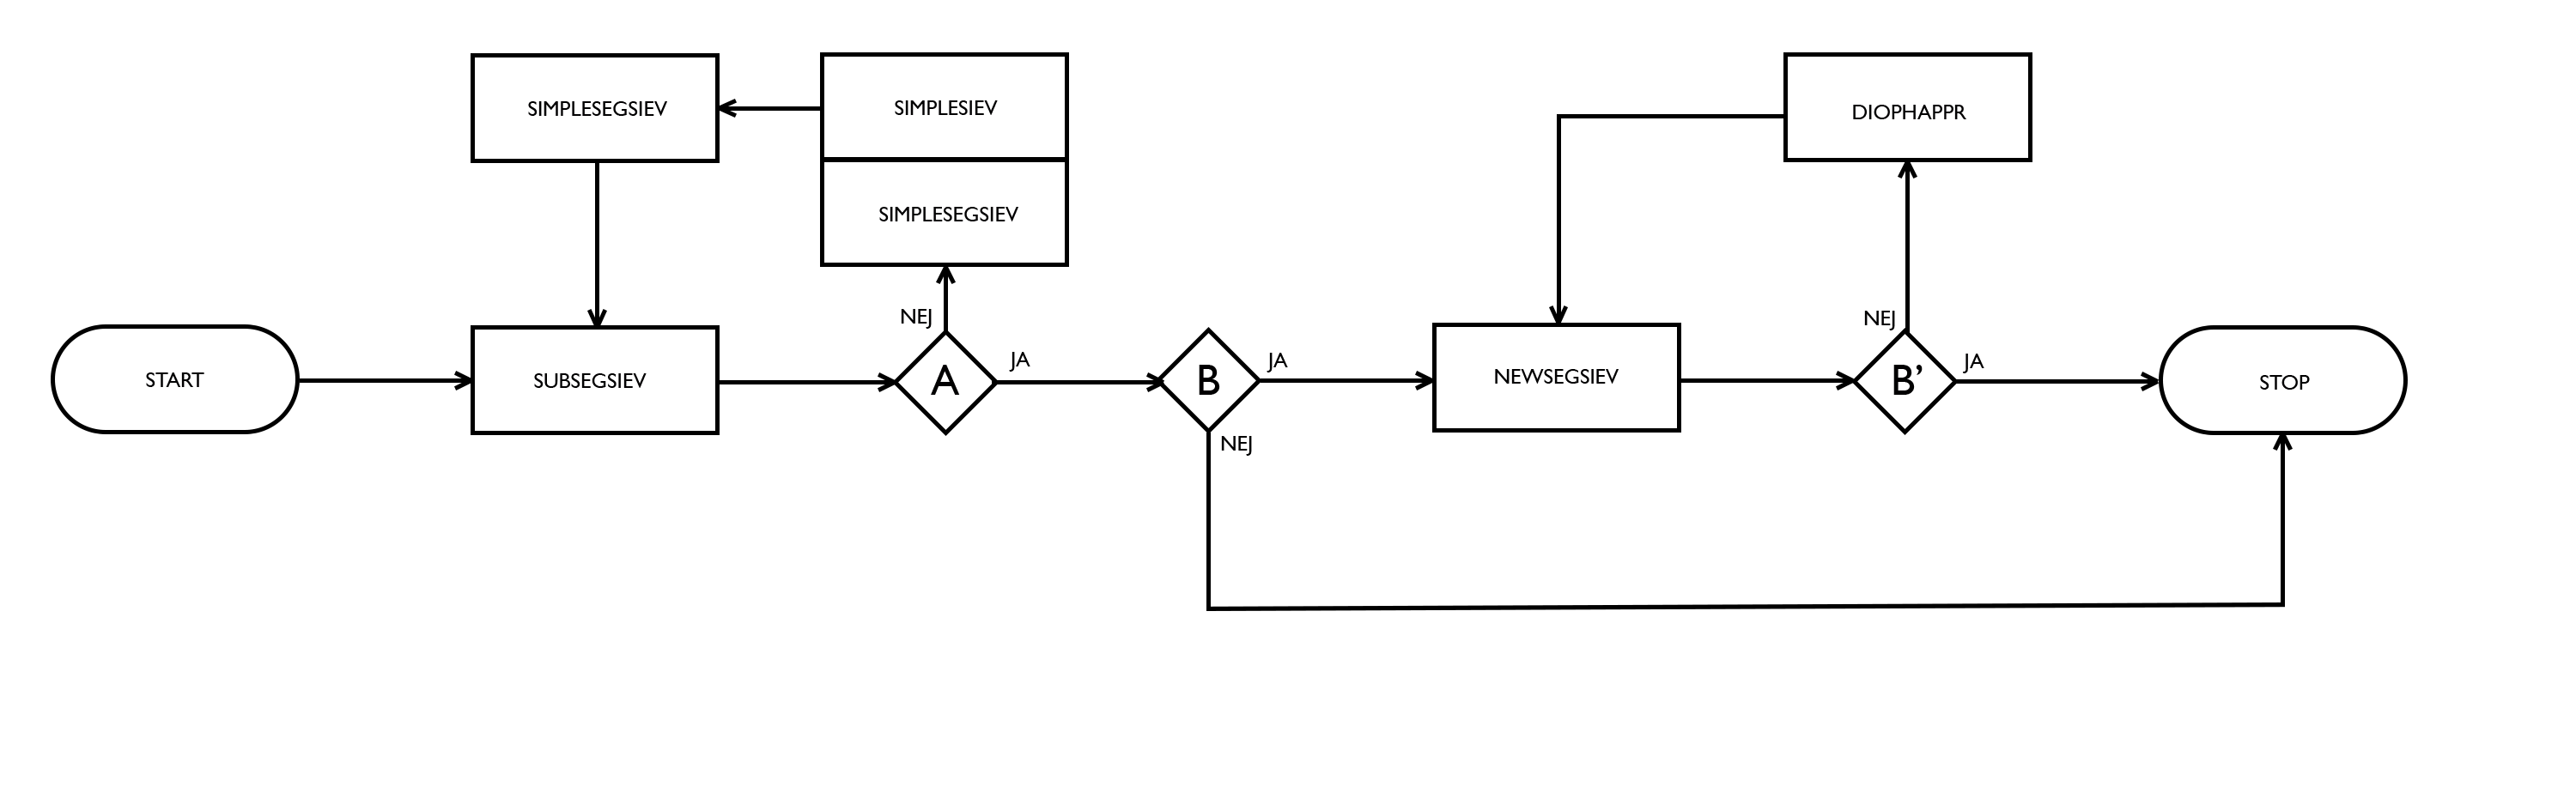
\includegraphics[width = \textwidth]{erik/Images/flowchart_v2.1.png}
    \usetikzlibrary{shapes.geometric, arrows, positioning}


\def\H{0.9cm}       % Min height for all objects
\def\W{2.15cm}      % Min width of rectangles
\def\Wpill{1.6cm}   % Min width of pills
\def\Wsplit{2.15cm} % Min width for split box (ugly solution)
\def\distV{1.4cm}   % Vertical distance between objects
\def\distH{0.6cm}   % Horizontal distance between objects


% Style
%\tikzstyle{every node} = [font=\tiny]
\tikzstyle{every node} = [font=\scriptsize]
\tikzstyle{every path} = [thick]
\tikzstyle{arrow} = [thick,->,>=stealth]

% Objects
\tikzstyle{startstop} = [rectangle, minimum width=\Wpill, minimum height=\H, text centered, draw=black, rounded corners=\H/2]
\tikzstyle{process}   = [rectangle, minimum width=\W, minimum height=\H, text centered, draw=black]
\tikzstyle{decision}  = [diamond,   minimum width=\H, minimum height=\H, text centered, draw=black]


{\fontfamily{qhv}\selectfont % phv, qhv eller qag 
\begin{tikzpicture}
% Objects
    % Start
    \node (start) [startstop]                       {\textsc{start}};
    % First loop
    \node (sub)   [process,  right=\distH of start] {\textsc{SubSegSiev}};
    \node (sim2)  [process,  above=\distV of sub]   {\textsc{SimpleSegSiev}};

    \node (sim1)  [process,  right=\distH of sim2, minimum width=\Wsplit]  {\textsc{SimpleSiev}};
    \node (sim0)  [process,  below=-\pgflinewidth of sim1, minimum width=\Wsplit]  {\textsc{SimpleSegSiev}};
    \node (A)     [decision, below=\distV of sim1]  {\textbf{A}};
    % Middle
    \node (B0)    [decision, right=\distH + 0.5cm of A]     {\textbf{B}};
    % Second loop
    \node (new)   [process,  right=\distH of B0]    {\textsc{NewSegSiev}};
    \node (B1)    [decision, right=\distH of new]   {\textbf{B'}};
    \node (dio)   [process,  above=\distV of B1]    {\textsc{DiophAppr}};
    % Stop
    \node (stop)  [startstop,right=\distH of B1]    {\textsc{stop}};

% Arrows
    % Start to first loop
    \draw [arrow] (start) -- (sub);
    % First loop
    \draw [arrow] (sub)   -- (A);
    \draw [arrow] (A)     -- (sim0);
    \draw [arrow] (sim1)  -- (sim2);
    \draw [arrow] (sim2)  -- (sub);
    % Middle
    \draw [arrow] (A)     -- (B0);
    \draw [arrow] (B0)    -- (new);
    \draw [arrow] (B0)    |- ([yshift=-\distV]B0.south) -| (stop);
    % Second loop
    \draw [arrow] (new)   -- (B1);
    \draw [arrow] (B1)    -- (dio);
    \draw [arrow] (dio)   -| (new);
    \draw [arrow] (B1)    -- (stop);

% Decision texts
    \node[above=3pt of A,  anchor=east]  {NEJ};
    \node[right=4pt of A,  anchor=south] {JA};
    \node[below=3pt of B0, anchor=west]  {NEJ};
    \node[right=4pt of B0, anchor=south] {JA};
    \node[above=3pt of B1, anchor=east]  {NEJ};
    \node[right=4pt of B1, anchor=south] {JA};
\end{tikzpicture}
}
\vspace{0.5cm}
    \caption{Ett övergripande flödesschema för algoritmen \textsc{NewSegSiev}. Observera att det finns två huvudloopar i algoritmen, en där kriterium A är uppfyllt då intervallet \([n - \Delta, n + \Delta]\) sållats med alla primtal \(p \leq K \Delta\) och den andra där kriterium B' är uppfyllt då algoritmen sållat för resterande tal upp till \(\sqrt{n + \Delta}\). Slutligen är kriterium B i koden identiskt med B' men illustrerar i flödesschemat möjligheten för programmet att aldrig gå in i den andra loopen då \(\Delta > \sqrt{n + \Delta}/K\).}
    \label{fig:flowchart}
\end{figure}


%Målet med \textsc{SubSegSiev} är att, givet \(n, \Delta \) och $M$, sålla \([n, n + \Delta]\) med primtal $p \leq M$. Algoritmen gör detta på i stort sett samma vis som i Eratosthenes klassiska såll men delar in primtalen i segment för att optimera minneskomplexiteten. \todo{Fortsätt med att gå igenom SimpleSiev, SimpleSegSiev och SubSegSiev och kort förklara hur de samverkar i NewSegSiev}.

Nästa steg, huvudalgoritmen i \textsc{NewSegSiev}, kräver mer matematisk eftertanke. Uppgiften som kvarstår för funktionen efter \textsc{SubSegSiev} är att sålla intervallet \([n - \Delta, n + \Delta]\) med resterande primtal, \( p \geq K \Delta\) där \(K \geq 5/2\). Problemet är löst genom att leta efter alla multiplar av \(m \geq K \Delta\) i vårt intervall. Låt \(\ell m\) vara en sådan multipel, då ser vi att
\begin{align} \label{alg.problem}
    n - \Delta \leq \ell m \leq n + \Delta \Longleftrightarrow 
    - \frac{\Delta}{m} \leq \frac{n}{m} - \ell \leq \frac{\Delta}{m} \Longleftrightarrow \left\{ \frac{n}{m} \right\} \in \left[- \frac{\Delta}{m}, \frac{\Delta}{m} \right] \bmod 1,
\end{align}
där $\big[- \frac{\Delta}{m}, \frac{\Delta}{m} \big] \bmod 1 = \bigcup_{k \in \mathbb{Z}} \big[k - \frac{\Delta}{m}, k + \frac{\Delta}{m} \big]$. Med den här presentationen av problemet gör \cite{HaraldSieve} två approximationer -- först en Taylorutveckling och därefter en diofantisk approximation. 

Den första approximationen syftar till att ersätta hyperbeln \(f(m) := \frac{n}{m}\) med en (diskontinuerlig) mängd tangenter till kurvan givna av en Taylorapproximation vid olika punkter \(m_0\),
\begin{align*}
    f(m) = f(m_0 + r) = \frac{n}{m_0} - \frac{n}{m_0^2} r + O\left(\frac{n}{m_-^3} r^2 \right)
\end{align*} % mellansteg nödvändigt?
där \(m_- = \min(m, m_0)\). Eftersom hyperbeln planar ut för större $m$ så kan vi approximera större och större intervall av kurvan med samma linjesegment utan att förstora feltermen. Mer specifikt så låter \cite{HaraldSieve} approximera kurvan med tangenter till kurvan på mitten, $m_0$, av intervallet \([M_i, M_i + 2R_i]\) där  $M_{i + 1} = M_i + 2R_i + 1$ med $M_0 = \lfloor K \Delta \rfloor + 1$ och
\begin{align*}% Eventuellt i stycke?
    R_i = \left\lfloor \sqrt{\Delta/(4n)} M_i \right\rfloor .
\end{align*}
Vi delar in kurvan i segment \([M, M + 2R]\) tills vi har täckt alla tal \(m \in [  \lfloor K \Delta \rfloor + 1, \sqrt{n + \Delta}]\). Orsaken till att \cite{HaraldSieve} väljer att definiera \(M, m_0\) och \(R\) som ovan är så att restermen inte övertar storleken på intervallet, med andra ord är resttermen \(\lesssim nr^2/m_-^3 \leq nR^2/M^3 = \Delta / (4M)\). Tar vi hänsyn till feltermen i problemformuleringen, (\ref{alg.problem}), så har vi omformulerat problemet till att hitta \(r \in [-R, R]\) så att \(P(r) = (\frac{n}{m_0} - \frac{n}{m_0^2} r) \in [-5\Delta/(4M), 5\Delta/(4M)] \bmod{1}\). Helfgotts val av \(K \geq 5/2\) fyller nu två syften: \(R \geq 1\) så att intevallen vi söker i inte är tomma och \(5\Delta/(4M) < 1/2\) så att intervallet vi försöker pricka inte är hela \(\mathbb{R}\).

Vi kan ställa ytterligare krav på \(r \in [-R, R]\) för att slippa gå över hela intervallet. Vad \cite{HaraldSieve} gör är att hitta en approximation för \(\alpha_1 := -n/m_0^2\) på formen \(a/q\) där $a,q$ är två relativt prima heltal med ett krav på nämnaren, $q \leq 2R$. Detta är precis funktionen av en så kallad diofantisk approximation och för att förstå den här processen krävs förkunskaper om kedjebråk som kan hittas i appendix \ref{APDX:cfrac}. Med kedjebråksnotationen från appendix så vill vi omformulera \(\alpha_1\) till ett enkelt kedjebråk, \(\langle a_0, a_1, \dots \rangle\). Följer vi algoritmen i \cite[sats 21.5]{Lindahl} så ges \(a_0\) av \(\lfloor \alpha_1 \rfloor\) och om inte \(\alpha_1\) var ett heltal, i vilket fall vi är färdiga, så blir resten \(0 < \alpha_1 - a_0 < 1\). Detta ger oss \(\xi_1 := 1 / (\alpha_1 - a_0) > 1\) och vi kan återupprepa samma steg: låt \(a_1 = \lfloor \xi_1 \rfloor\) och \(\xi_2 := 1 / (\xi_1 - a_1) > 1\). På så vis, om vi fortsätter, får vi en algoritm som genererar ett enkelt kedjebråk. 

%Det är förstås viktigt att veta att algoritmen har ett slut och för att se detta studerar vi konvergenterna \(c_n = p_n / q_n\). 
Vi kan vara säkra på att algoritmen slutar av sig självt eftersom vi utvecklar kedjebråket av ett rationellt tal, \(\alpha_1 = - n / m_0^2\), som därav är ett ändligt kedjebråk (se \cite[sats 21.5]{Lindahl}) men vi vill sannolikt avbryta processen redan tidigare. Vårt mål är att hitta en rationell approximation till \(\alpha_1\) med nämnare \(q \leq 2R\) och eftersom \((q_n)_{n>0}\) är en växande följd så kan vi välja att stoppa algoritmen när \(q_n \leq 2 R\) men \(q_{n + 1} > 2R\). Del 2 av sats \ref{app.kovfel} garanterar att vår approximation blir bättre för varje iteration och, för sådant $n$, så är \(\abs{\alpha_1 - \frac{a}{q}} \leq \frac{1}{q \cdot 2R}\). Till sist observerar vi att konvergenterna, \(p_n, q_n\), är relativt prima då del 2 av sats \ref{app.konvergenter} ger oss att \((p_{n-1}, q_{n-1})\) är en heltalslösning till den diofantiska ekvationen
\begin{align*}
    a x + b y = 1 \quad \text{ där }\ a = \pm q_n, b = \mp p_n
\end{align*}
vilket endast är möjligt om \(1\) är en multipel av största gemensamma nämnaren, \(\gcd{a,b}\), (ett resultat från elementär talteori, se förslagsvis \cite[sats 3.1]{Lindahl}). % H.L. istället för 1:a

Ovanstående algoritm heter \textsc{DiophAppr} i \cite{HaraldSieve} vilken beräknar en diofantisk approximation \(a / q\) av den ledande koefficienten \(\alpha_1\) i \(P(r)\) med kravet på $q$ som vi nämnde tidigare. Algoritmen returnerar täljare och nämnare separat samt passar på att beräkna \(a^{-1} \pmod{q}\) då del 2 av sats \ref{app.konvergenter} ger oss en möjlighet att räkna ut inversen i termer av konvergenterna. 

Målet med att introducera \textsc{DiophAppr} är så att vi kan gå från att leta lösningar till (\ref{alg.problem}) i \(r \in [-R, R]\) till att endast leta bland ett urval av heltal. Vi har redan hittat en rationell approximation av \(\alpha_1\) och, konstantkoefficienten av \(P(r)\), \(\alpha_0 := n / m_0\) kan vi också approximera med bråket \(\lfloor \alpha_0 q + 1/2 \rfloor / q := c / q\). Således ser vi att
\begin{align*}
    \abs{q \cdot P(r) - (c + ar)} &= \abs{\left(\alpha_1 - \frac{a}{q}\right) q r + \left( \alpha_0 q - c\right)} \leq 
    \abs{\alpha_1 - \frac{a}{q}} q \abs{r} + \abs{\alpha_0 q - c} \\
    &\leq \frac{1}{q \cdot 2R} \cdot qR + \frac{1}{2}  = 1
\end{align*}
tack vare noggrannheten av den diofantiska approximationen, hur vi definierade \(c\) och att \(r \in [-R, R]\). Därav, om \(P(r) \in [-5\Delta/(4M), 5\Delta/(4M)] \bmod 1\) så medför det att
\begin{align*}
    c + ar \in \{- k - 1, - k, ... , k, k + 1\} \bmod q
\end{align*}
där \(k = \lfloor q \cdot 5\Delta/(4M) \rfloor\). Det räcker alltså att sålla för \(r \equiv - a^{-1} (c + j) \pmod{q}\) för heltal \(j \in [-k-1, k+1]\), där den multiplikativa inversen av $a \pmod{q}$ tillhandahålls av \textsc{DiophAppr}. 

% Detta kan ge falska lösningar, vi kan kontrollera detta --> villkor på display-rad
Vi har alltså sett hur \cite{HaraldSieve} först sparar minnesplats genom att segmentera första delen av algoritmen och sedan tid i andra delen genom att vara selektiv med vilka tal som vi sållar bort multiplar av. I det senare fallet finns som mest en multipel i intervallet, per konstruktion av \(K \Delta\), och vi har visat att alla \(m = m_0 + r\) med en multipel i intervallet har \(r \equiv - a^{-1} (c + j) \pmod{q}\), för \(a, c, j\) definierade ovan. Däremot har vi inte visat det motsatta och det kan vara så att vissa \(r\) som genereras är falska lösningar orsakade av Taylor- och den diofantiska approximationen. Därför behöver vi också kontrollera att multipeln av \(m\) ingår i intervallet, det vill säga att
\begin{align} \label{alg.control}
    \ell m %:= \lfloor (n + \Delta) / m \rfloor \cdot m 
    \in [n - \Delta, n + \Delta] \quad \text{och } \quad  \ell m > m.
\end{align}

I nästa avsnitt kommer vi se vilka val som gick in i Python-implementationen av pseudokoden samt studera tidsbesparingar och möjliga förbättringar från originalalgoritmen.

%till den diofantiska approximationen \(a/q\) för \(\alpha_1\) så att \(\abs{\alpha_1 - \frac{a}{q}} \leq \frac{1}{q \cdot 2R}\) för största möjliga konvergent $q$ mindre än eller lika med \(2R\). \textsc{DiophAppr} 